%---------------------导言区---------------------------%
\documentclass[12pt,a4paper,UTF8]{ctexart}
\usepackage{geometry}
	\geometry{left=2.5cm,right=2.5cm,top=3.2cm,bottom=2.8cm}
\usepackage{xeCJK,amsmath,paralist,enumitem,booktabs,multirow,graphicx,subfig,setspace,listings,lastpage,hyperref}
	\setlength{\parindent}{2em}
	\lstset{language=Python}
\usepackage{fancyhdr}
	\pagestyle{fancy}
	\rhead{B9 迈克耳孙干涉仪及其应用(白光干涉)}
	\lhead{基础物理实验\uppercase\expandafter{\romannumeral2}实验报告}
	\cfoot{Page \thepage/\pageref{LastPage}}  %当前页\总页数
	\rfoot{\today}
	\renewcommand{\headrulewidth}{0.4pt}
	\renewcommand{\theenumi}{(\arabic{enumi})}

%%%%%%%%%%%%%%%%%%%%%%%%%%%%%%%%%%%%%%%%%%%%%%%%%%%%%%%%%%
%%%%%%%%%%%%%%%%%%%%%%%%%正文开始%%%%%%%%%%%%%%%%%%%%%%%%%%
%%%%%%%%%%%%%%%%%%%%%%%%%%%%%%%%%%%%%%%%%%%%%%%%%%%%%%%%%%

\begin{document}

%%begin-------------------标题与信息-----------------------%%
%%标题
\begin{center}
\LARGE\textbf{B9 迈克耳孙干涉仪及其应用(白光干涉)}
\end{center}

%%信息
\begin{doublespacing}
	\centering
	\begin{tabular}{ll}
	 & \\
	{\CJKfontspec{Droid Sans Fallback} 实验人:黄子维 20980066} & {\CJKfontspec{Droid Sans Fallback}合作者:黄睿杰 20980062}\\
	{\CJKfontspec{Droid Sans Fallback} 实验时间:2021.9.23~星期四~上午} & {\CJKfontspec{Droid Sans Fallback} 室温:29$^{\circ}$C~相对湿度:62\%}
	\end{tabular}
\end{doublespacing}
%%end-------------------标题与信息-----------------------%%

\subsection*{【实验目的】}
	\begin{enumerate}[label=\arabic*.]
		\item 观察等倾、等厚干涉现象及调节白光干涉条纹。
		\item 学习用迈克耳孙干涉仪测量钠光谱波长差的方法。
		\item 学习用白光干涉测量透明薄片折射率的方法。
	\end{enumerate}

\subsection*{【仪器用具】}
    \begin{table}[htbp]
        \centering
        \begin{tabular}{cccp{20em}}
        \toprule
        编号    & 仪器用具名称 & 数量    & 主要参数(型号,测量范围,测量精度等) \\
        \midrule
        1	&精密干涉仪	&1	&KF-WSM	\\
		2	&He-Ne激光器	&1	& /	\\
		3	&钠钨双灯	&1	& /	\\
        4	&透明薄片	&1	& /	\\
		\bottomrule
        \end{tabular}%
        \label{tab:device}%
    \end{table}%

\subsection*{【实验原理】}
    \subsubsection*{1. 测量钠双黄线的波长差}
    钠黄光含有两种波长相近的光。
    \paragraph*{光拍现象} 采用钠灯作光源,在干涉仪动镜移动过程中,干涉条纹会出现清晰与模糊的周期性变化。
    \paragraph*{钠双黄线的波长差} 干涉条纹出现一次模糊$\to$清晰$\to$模糊的变化时,$M_1$镜移动的距离为$\Delta d$,则钠双黄线波长差为:
    
	$$
    \Delta \lambda = \frac{\bar\lambda^2}{2\Delta d}
    $$

    \subsubsection*{2. 利用白光干涉测定透明薄片的厚度或折射率}
    \paragraph*{白光等厚条纹}
    \newline
    \indent
    \begin{itemize}
			\item 先采用激光光源,调节出等倾干涉圆环,再减小两反射臂的光程差,直至等倾圆环几乎消失,此时两臂光程差相等。
			\item 换上扩散的白光光源,并微调可调反射镜的倾斜度,则可在视场中观察到彩色的条纹,此即为白光等厚干涉条纹。
			\item 缓慢移动$M_1$镜,使中心暗纹移到视场中央。中心暗纹:彩色条纹中间的全黑条纹。
		\end{itemize}
    \paragraph*{测量薄片折射率}
    \newline
    \indent
    \begin{enumerate}[label=\arabic*.]
        \item 放置薄片:在$M_1$镜和$G_1$镜间平行放置厚度为$t$,折射率为$n$的透明薄片,则光程差增大$\Delta L=2t(n-1)$
        \item 补偿光程:向$G_1$镜方向移动$M_1$镜,当移动距离$\Delta d = \frac{\Delta L}{2}$时,光程差被补偿,中心暗纹和彩色条纹重新出现,则$\Delta d = t(n-1)$
    \end{enumerate}	

\subsection*{【实验装置】}
	\subsubsection*{1. 迈克耳孙干涉仪光路图}
		光路图如图\ref{fig:illus-1}所示。测定钠双黄线波长差时,应将氦氖激光器换成钠光源并移去观察屏和薄片。测定薄片折射率时,应将氦氖激光器换为白光光源并移去观察屏。
		\begin{itemize}
			\item $M_1$:可移动反射镜
			\item $M_2$:固定反射镜
			\item $G_1$:分光镜
			\item $G_2$:补偿镜
		\end{itemize}
		\begin{figure}[htbp]
			\centering
			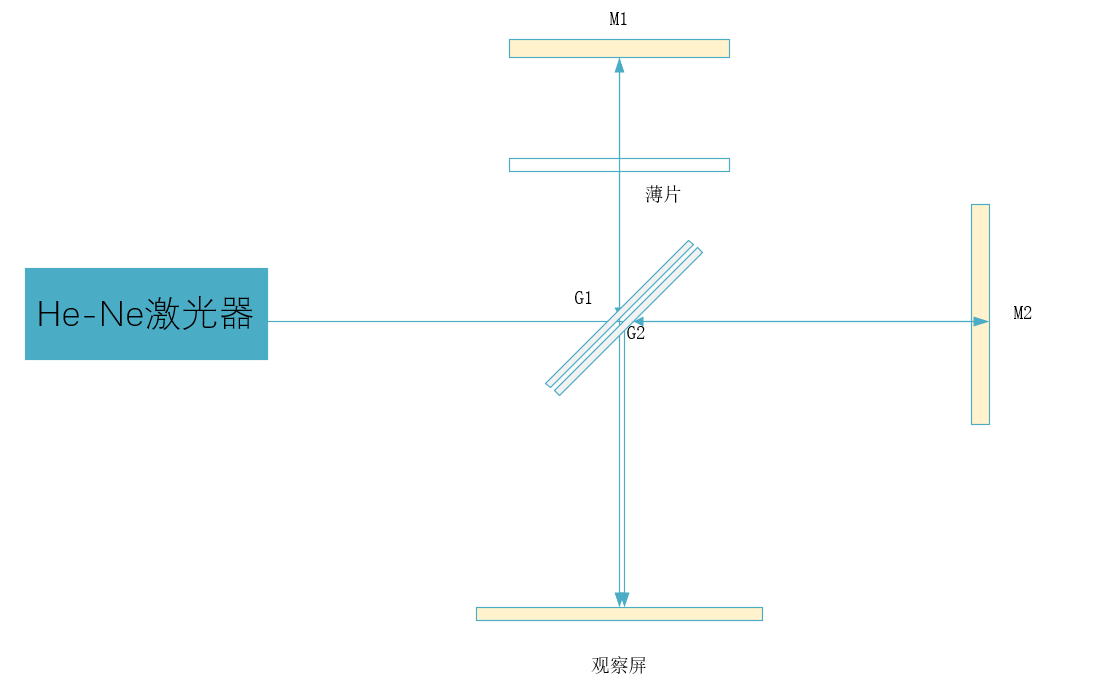
\includegraphics[width=0.7\textwidth]{attachments/illus-1.png}
			\caption{迈克耳孙干涉仪}
			\label{fig:illus-1}
		\end{figure}

		
		
\subsection*{【实验内容及步骤】}
	\subsubsection*{1. 用氦氖激光器调出等倾干涉图像}
		\begin{itemize}
			\item 安装干涉仪,扩束镜先不安装。
			\item 调节$ He-Ne $激光器的高度和倾斜度,使激光束从分束镜的中心人射。
			\item 调节$M_1$和$M_2$反射镜的倾斜度调节螺钉,使各镜面的入射和出射点高度与分束镜接近,$M_1$和$M_2$反射的光点在观察屏中央重合。
			\item 装上扩束镜,观察干涉条纹。
		\end{itemize}
	\subsubsection*{2. 测量钠双黄线波长差}
		\begin{enumerate}[label=\arabic*.]
			\item 用$ He-Ne $激光,调出干涉圆环。移动反射镜$M_1$,使条纹变宽变稀,至观察屏上只有少数几个圆环,此时两干涉臂的光程几乎相等。
			\item 改用灯前装有毛玻璃的钠灯,拆除观察屏。
			\item 肉眼观察,仔细调节$M_2$镜的倾斜度调节螺钉和$M_1$镜的位置,可观察到黄黑相间的直线状等厚干涉条纹。
			\item 调节移动$M_1$镜,观察条纹模糊$\to$清晰$\to$模糊的周期变化过程,记录每周期移动距离$\Delta d$,依此计算钠双黄线波长差。
		\end{enumerate}

	\subsubsection*{3. 白光干涉的调节并测透明薄片的折射率}
		\begin{enumerate}[label=\arabic*.]
			\item 用$ He-Ne $激光,调出干涉圆环。移动反射镜$M_1$,使条纹变宽变稀,至观察屏上只有少数几个圆环,此时两干涉臂的光程几乎相等。
			\item 改用灯前装有毛玻璃的汞灯,拆除观察屏。
			\item 肉眼观察,仔细调节$M_2$镜的倾斜度调节螺钉和$M_1$镜的位置,可观察到彩色的直线状等厚干涉条纹。
			\item 在分束镜和动镜间垂直光路安装透明薄片,彩色条纹消失。缓慢调节精密测微头,缩小$M_1$和$G_1$之间的距离,重新观察到彩色条纹,记录$M_1$移动的距离$\Delta d$
			\item 用螺旋测微计测量薄片的厚度$t$,计算薄片的折射率。
		\end{enumerate}


\subsection*{【数据处理及分析】}
	\subsubsection*{1. 测量钠双黄线波长差}
		条纹模糊$\to$清晰$\to$模糊周期中$M_1$移动的距离$\Delta d$为(mm):
		
		$$
		[0.305,0.275,0.305,0.280,0.275,0.305,0.290,0.285,0.295,0.295]
		$$

		平均值为$\Delta d = 0.291 mm$,标准差为$0.012mm$。取$\bar\lambda = 589.3nm$,代入公式$\Delta \lambda = \frac{\bar\lambda^2}{2\Delta d}$计算得$\Delta \lambda = 0.597nm$

		不确定度$S = 0.027nm$,故

		$$
		\Delta \lambda = 0.597 \pm 0.027 nm
		$$

	\subsubsection*{2. 白光干涉的调节并测透明薄片的折射率}

		\paragraph{测量薄片厚度}~
		\newline
		\indent
		薄片厚度测量值(mm):
		
		$$
		[0.160,0.151,0.185,0.154,0.152]
		$$

		平均值$t = 0.160mm$,标准差$0.014mm$

		\paragraph{利用白光干涉测量薄片折射率}~
		\newline
		\indent
		白光干涉的中心暗条纹实验结果如图\ref{fig:illus-2}
		\begin{figure}[htbp]
			\centering
			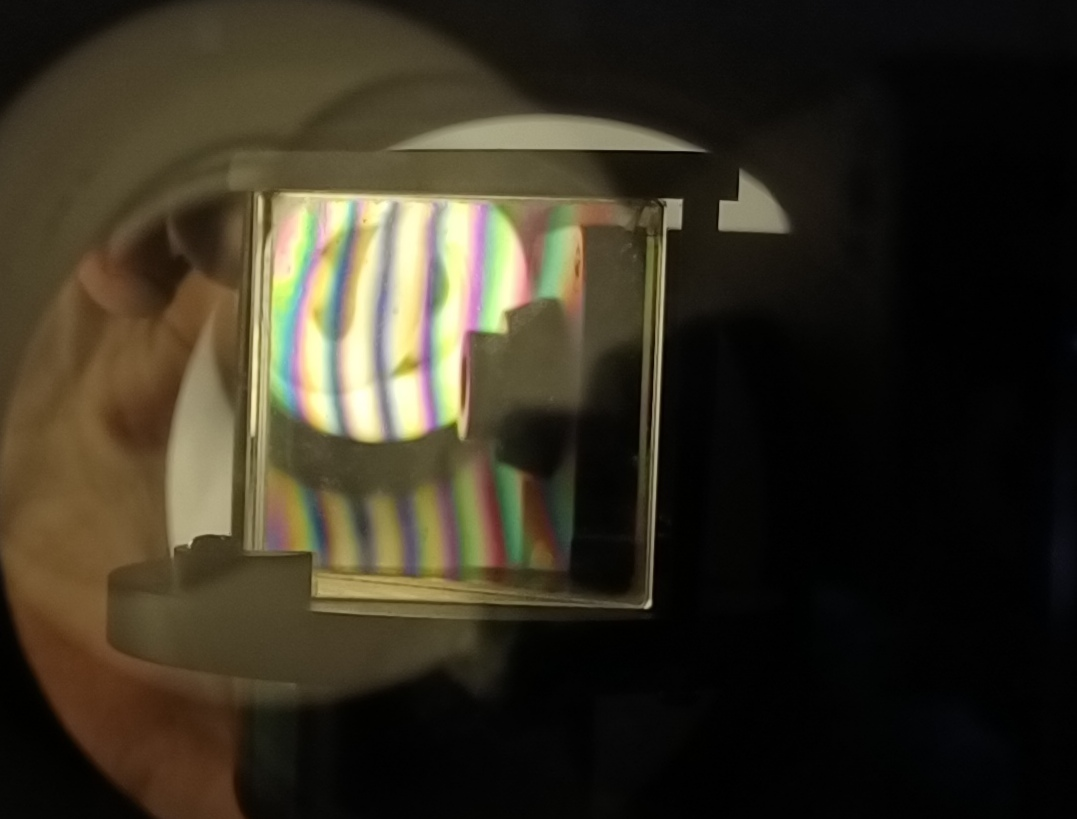
\includegraphics[width=0.5\textwidth]{attachments/illus-2.jpg}
			\caption{中心暗条纹}
			\label{fig:illus-2}
		\end{figure}

		实验结果如表\ref{tab:1}
		\begin{table}[htbp]
			\centering
			\begin{tabular}{|l|l|l|l|l|l|l|}
			\hline
			EXP & 放置薄片后$M_1$位置/mm & 放置薄片前$M_1$位置/mm & 距离差值/mm \\ \hline
			1 & 12.320 & 12.398 & 0.078 \\ \hline
			2 & 12.318 & 12.399 & 0.081 \\ \hline
			3 & 12.321 & 12.396 & 0.075 \\ \hline
			\end{tabular}
			\caption{放置薄片前后出现干涉条纹所对应$M_1$镜位置以及差值}
			\label{tab:1}
		\end{table}

		$\Delta d$平均值为$0.078mm$,标准差为$0.003mm$。
		
		代入$n = \frac{\Delta d}{t}+1$计算得$n = 1.486$

		不确定度$S = 0.062$,故
		$$
		n = 1.486 \pm 0.062
		$$

		

\subsection*{【思考题】}
	\subsubsection*{1. 如何测量透明溶液的折射率?请提出实验方案并说明其合理性。}
		答:旋转样品法。
		\begin{enumerate}[label=\arabic*.]
			\item 组装迈克耳孙干涉仪,将可固定在旋转底座上的方形透明液槽置于动镜$M_1$和分束镜$G_1$之间。液槽宽度为$t$		
			\item 分别进行空槽与装液两次实验,两次实验转动相同角度,分别记录条纹变化数$\Delta N_1$和$\Delta N_2$,则修正后的条纹变化数为$\Delta N=\Delta N_1-\Delta N_2$
			\item 则 $n = \frac{tsin^2\theta}{2t(1-cos\theta)-\Delta N \lambda}+ (1-cos\theta-\frac{\Delta N \lambda}{2t})$
		\end{enumerate}
		合理性:由于透明溶液需要容器装载,而容器壁将会引入额外光程差,因此设计空槽与装液两次实验,得到修正的条纹变化数,将能够消除这部分误差,提高结果准确性。
	\subsubsection*{2. 当空气的温度改变时,空气的折射率也会改变的,怎样去测量空气的折射率?}
		答:利用恒温装置控制温度,利用迈克耳孙干涉仪分别测定在不同温度下空气的折射率,测得多组数据后拟合空气折射率随温度变化关系曲线,外推得到特定温度对应的空气折射率。


\subsection*{【项目源码】}
\url{https://github.com/Jeg-Vet/SYSU-PHY-EXP/tree/main/B9-%20Michelson_interference_II}
		
\end{document}
